\documentclass[journal,twoside,web]{ieeecolor}
\usepackage{generic}
\usepackage{cite}
\usepackage{amsmath,amssymb,amsfonts}
\usepackage{algorithmic}
\usepackage{graphicx}
\usepackage{textcomp}
% \def\BibTeX{{\rm B\kern-.05em{\sc i\kern-.025em b}\kern-.08em
%     T\kern-.1667em\lower.7ex\hbox{E}\kern-.125emX}}
% \markboth{\journalname, VOL. XX, NO. XX, XXXX 2017}
% {Author \MakeLowercase{\textit{Kulas, Ahmed, Ozara}}: Final project report: ECE 657A- Data and Knowledge Modelling and Analysis (April 2019)}
\begin{document}
\title{Santander Customer Transaction Prediction (March 2019)} \\

\author{Adam Kulas, Ammar Ahmed, and Richard Ozara\\
\institute University of Waterloo,ON N2L 3G1, Canada\\akulas@uwaterloo.ca\\
a272ahme@uwaterloo.ca \\\centerline{roozara@uwaterloo.ca}}

\maketitle



\begin{abstract}
Kaggle is a popular platform for companies and researchers to post interesting datasets and benefit from a crowd sourced approach to machine learning. We will describe the process and detailed steps to attempt to solve a binary classification problem presented by Santander bank and Kaggle. This paper first sets a baseline using different machine learning algorithms and compares them to one another. Different techniques are explored to improve on the initial baseline such as Bayesian search, sampling techniques and ensembling. 
\end{abstract}

\begin{IEEEkeywords}
Binary classification, Ensembling, gradient boosting, Machine learning, Naive Bayes, lgbm, logistic regression, XGBoost
\end{IEEEkeywords}


%%%%%%%%%%%%%%%%%%%%%%%%%%%%%%%%%%%%%%%%%%%%%%%%%%%%%%%%%%%%%%%%%%%%%%%%%%%%%%%%%%%%%%%%%%%%%%%%%%%%%%%%
% INTRODUCTION
%%%%%%%%%%%%%%%%%%%%%%%%%%%%%%%%%%%%%%%%%%%%%%%%%%%%%%%%%%%%%%%%%%%%%%%%%%%%%%%%%%%%%%%%%%%%%%%%%%%%%%%%

\section{Introduction}
\label{sec:introduction}
\IEEEPARstart{T}{he} purpose of this project is to solve a problem presented by the company Santander. Santander is a bank that is originating in Spain. Since 2013 they have been serving customers in northeastern North America. Santander mentions in the competition description that their most common problems are binary classification problems. The main goal for the competition is to predict which customers will make a specific transaction in the future, irrespective of money transacted. The problem presented by this challenge is a binary classification problem. The challenge is hosted on Kaggle's official website where competitors submit their predicted results online. The key metric for evaluation in this competition is the Receiver Operating Characteristics Area Under The Curve (AUCROC) between the predicted probability and the observed target. The approach followed in this paper started with data preprocessing and then to data exploration and visualization. After that, a simple random forest model was created to set a baseline performance bench-mark and to help with extracting important features as part of the exploratory data analysis (EDA). Then, implemented supervised machine learning classffication algorithms such as Naive Bayes and logistic regression that were more specifically tailored to the dataset and problem space. Lastly, a more advanced models were tested such XGBoost and LGBM which required a lot of exploring and tuning their hyperparamters. Also, techniques such ensembling models were tested and all results were compared and evaluated. Throughout the process of testing those models, cross-validation CV was performed and cross-referenced with kaggle leader board scores. The overall aim of the paper is to present the information and results in our journey to maximize our Leader Board (LB) score for the competition.

\subsection{Abbreviations and Acronyms}

CV score = Cross Validation score \\
XGBoost = Extreme Gradient Boosting  \\
LGBM = Light Gradient Boosting Model \\
PCA = Principal Component Analysis \\
AUC = Area Under the Curve \\
ROC = Receiver Operator Characteristics \\
SMOTE = Synthetic Minority Oversampling Technique \\
Hyperopt = Distributed Asynchronous Hyper-parameter Optimization.

%%%%%%%%%%%%%%%%%%%%%%%%%%%%%%%%%%%%%%%%%%%%%%%%%%%%%%%%%%%%%%%%%%%%%%%%%%%%%%%%%%%%%%%%%%%%%%%%%%%%%%%%
% Description of the data
%%%%%%%%%%%%%%%%%%%%%%%%%%%%%%%%%%%%%%%%%%%%%%%%%%%%%%%%%%%%%%%%%%%%%%%%%%%%%%%%%%%%%%%%%%%%%%%%%%%%%%%%

\section{Description of the data}
The dataset used in this project is provided by Santander and can be downloaded from kaggle.com. There are two main files: "train.csv" which contains the training set and the "test.csv" which contains the test set. The size of the "train.csv" is 200k x 201 (40,200,000 data points) and for the "train.csv" is 200k x 202 (40,000,000 data points). The "train.csv" has the attributes: binary target column, string ID\_code column, and the numeric feature variables (var0 till var 199) while the "test.csv" contains the string ID\_code and the numeric feature variables, so the task is to predict the value of target column in the test set.The train and test datasets are fully anonymized. Test labels (target) is private - predicted results must be submitted online and submissions are evaluated on area under the ROC curve .






%%%%%%%%%%%%%%%%%%%%%%%%%%%%%%%%%%%%%%%%%%%%%%%%%%%%%%%%%%%%%%%%%%%%%%%%%%%%%%%%%%%%%%%%%%%%%%%%%%%%%%%%
% LITERATURE REVIEW
%%%%%%%%%%%%%%%%%%%%%%%%%%%%%%%%%%%%%%%%%%%%%%%%%%%%%%%%%%%%%%%%%%%%%%%%%%%%%%%%%%%%%%%%%%%%%%%%%%%%%%%%
\section{Literature Review}

\subsection{Bayesian optimization}
The motivation for using an Bayesian optimizer is to optimize the model jointly which leads to improving the model outcome significantly~\cite{shahriari2016taking}. When building models to solve the binary classification problems, certain techniques may have many model parameters. XGBoost and LGBM are random forest classifiers that each have over 60 parameters to tune/optimize. Bayesian optimization techniques is one of the most powerful and efficient approaches adapted in terms of the number of function evaluations required~\cite{brochu2010tutorial}. As mentioned in ~\cite{brochu2010tutorial}, this efficiency is due to the fact that Bayesian optimization is able to incorporate prior belief about the problem to help direct the sampling, and to trade off the exploration and exploitation of the search space. Unlike Gridsearch optimization where it tries every single combination that results in improving the model outcomes. Gridsearch would have resulted in a tremendous computational power and time. For this reason Bayesian optimization was the optimal choice for our project. 

\subsection{SMOTE - Synthetic Minority Over-sampling Technique}
SMOTE is a technique for over-sampling in which the minority class is over-sampled by creating synthetic examples. The synthetic examples are generated in a less application-specific manner by in feature space and not the data space~\cite{chawla2002smote}. The approach for over-sampling minority class is by introducing synthetic examples to each minority class sample along the line segments joining any or all of the k minority class nearest neighbors~\cite{chawla2002smote}. Neighbors are randomly chosen from the k nearest nearest neighbors, depending on the amount of over-sampling needed~\cite{chawla2002smote}. 


%%%%%%%%%%%%%%%%%%%%%%%%%%%%%%%%%%%%%%%%%%%%%%%%%%%%%%%%%%%%%%%%%%%%%%%%%%%%%%%%%%%%%%%%%%%%%%%%%%%%%%%%
% Proposed Methodology - Strategy/Methodology (What was our plan)
%%%%%%%%%%%%%%%%%%%%%%%%%%%%%%%%%%%%%%%%%%%%%%%%%%%%%%%%%%%%%%%%%%%%%%%%%%%%%%%%%%%%%%%%%%%%%%%%%%%%%%%%
\section{Proposed Strategy/Methodology}
In order to develop a model and strategy that would perform well on the competition's data-set, a standard data science work flow was adopted. Multiple steps are common in the process of solving similar problems~\cite{tandel_2017}. These steps include: data cleaning, data exploration, initial models, feature engineering, and hyper-parameters tuning. It is important to mention that these steps are not immutable and change depending on the problem definition. Figure~\ref{fig:flowchart} shows the milestones of the project.



\begin{figure}[h!]
  \centering
  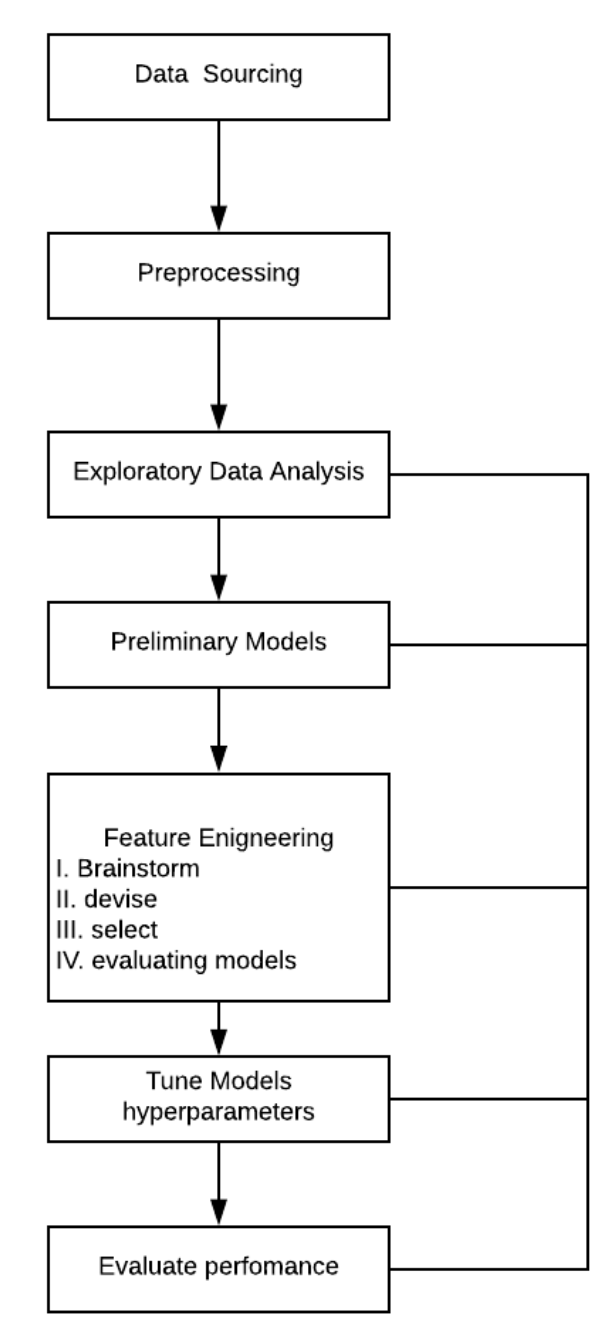
\includegraphics[width=2in]{flowchart.png}
  \caption{Flowchart representing steps in project execution}
  \label{fig:flowchart}
\end{figure}



%testing up sampling vs downsampling




                        %%%%%%%%%%%%%%%%%%%%%%%%%%%%%%%%%%%%%%%%%%%
                            % Subsection/ EDA
                        %%%%%%%%%%%%%%%%%%%%%%%%%%%%%%%%%%%%%%%%%%%
\subsection{Exploratory Data Analysis}
Exploratory data analysis (EDA) refers to the critical process of performing initial investigations on data so as to discover patterns,to spot anomalies,to test hypothesis and to check assumptions with the help of summary statistics and graphical representations ~\cite{patil_patil_2018}.



                %%%%%%%%%%%%%%%%%%%%%%%%%%%%%%%%%%%%%%%%%%%
                            % Subsection/ Key features of the chosen models
                        %%%%%%%%%%%%%%%%%%%%%%%%%%%%%%%%%%%%%%%%%%%

\subsection{Key features of the chosen models}
As stated earlier, benchmark models were first created. The first two models considered here were naive bayes and logistic regression. The reason behind the choice is because these two models are simple to implement as they have a minimal number of hyper-parameters tuning. Having a benchmark models helped in having a starting point and to get the feel of the dataset. The next two models considered where XGBoost and LGBM which are tree based learning algorithms. More high level explanation of these models is followed.  
                        %%%%%%%%%%%%%%%%%%%%%%%%%%%%%%%%%%%%%%%%%%%
                            % Subsection/ Naive Bayes classifier
                        %%%%%%%%%%%%%%%%%%%%%%%%%%%%%%%%%%%%%%%%%%%
                        
\subsubsection{Naive Bayes classifier}
Naive Bayes is a probabilistic machine learning model based on the Bayes theorem with an assumption of independence among the features.This  conditional independence  assumption  rarely  holds  true  in  real world  applications,  hence  the  characterization  as Naive yet the algorithm tends to perform well and learn  rapidly  in  various  supervised classification problems~\cite{dimitoglou2012comparison}. Main advantage of this model is that it can be easily trained on small datasets. Although the dataset used in this project is somewhat large, it was down-sampled (more explanation will be followed in the later section). Also, the data size was reduced further when splitting the down-sampled data into train and test. Both of these helped in providing the initial setup of having a good performing naive Bayes model. 

                        %%%%%%%%%%%%%%%%%%%%%%%%%%%%%%%%%%%%%%%%%%%
                            % Subsection/ Logistic Regression
                        %%%%%%%%%%%%%%%%%%%%%%%%%%%%%%%%%%%%%%%%%%%
                        
\subsubsection{Logistic Regression}
Logistic regression is a regression analysis that can be used for predictions when the target variable is dichotomous (binary). It is used to describe data and to explain the relationship between one dependent binary variable and one or more nominal, ordinal, interval or ratio-level independent variables ~\cite{statisticssolutions}. The advantage of logistic regression is that it is simple to implement with very few parameters.

                        %%%%%%%%%%%%%%%%%%%%%%%%%%%%%%%%%%%%%%%%%%%
                            % Subsection/ Boosting Algorithms
                        %%%%%%%%%%%%%%%%%%%%%%%%%%%%%%%%%%%%%%%%%%%
\subsection{Boosting Algorithms}
In order to understand XGBoost and lgbm functionally, the term gradient descent and gradient boosting had be understood first. 
Gradient descent, uses a cost function to measure how close the predicted values are to the actual values. It is desirable to have as little difference as possible between the predicted values and the actual values, other words, minimizing the cost function. This is done by associating weights with the trained models, therefore, the better weights associated with the model, the more accurate predicted outcome are and the lower the cost function as well. To summarize, gradient descent is an iterative optimization algorithm in which these associated weights are learned and then updated to minimize the cost function. \\
On the other hand, gradient boosting combines the principle of gradient descent and boosting to a supervised learning models. The idea of boosting is that a set of an ensemble of weak learners built where the wrongly predicted records are given a higher weights (boosted) so that the next model will pay more attention to those incorrectly classified labels and will try to predict them correctly. This technique converts a group of weak learners into a single strong learner.

                        %%%%%%%%%%%%%%%%%%%%%%%%%%%%%%%%%%%%%%%%%%%
                            % Subsection/ XGBOOST (eXtreme Gradient Boosting)
                        %%%%%%%%%%%%%%%%%%%%%%%%%%%%%%%%%%%%%%%%%%%
\subsubsection{XGBOOST- eXtreme Gradient Boosting}
XGBoost is a library for developing fast and high performance gradient boosting tree models and can be used as a standalone predictor. It is an advanced implementation of the gradient boosting algorithms. The main key features of XGBoost is scalability, which drives fast learning through parallel and distributed computing and offers efficient memory usage ~\cite{kdnuggets_analytics_big_data_data_mining_and_data_science}. There are several systems and algorithmic optimizations made on the XGBoost that made the scalability feature possible. This includes: a novel tree learning algorithm is for handling sparse data and a theoretically justified weighted quantile sketch procedure enables handling instance weights in approximate tree learning. XGBoost enables parallel and distributed computing which makes learning faster which enables quicker model exploration. More importantly, XGBoost take advantage of out-of-core computation and enables data scientists to process hundred millions of examples on a desktop. These were the main key features in choosing and testing XGBoost. 

                        %%%%%%%%%%%%%%%%%%%%%%%%%%%%%%%%%%%%%%%%%%%
                            % Subsection/ {LGBM (Light Gradient Boosting Model)
                        %%%%%%%%%%%%%%%%%%%%%%%%%%%%%%%%%%%%%%%%%%%
\subsubsection{LGBM- Light Gradient Boosting Model} 
Light GBM is a very high performing gradient boosting framework uses tree based learning algorithms that can be used for predictions, classifictions, ranking and many other machine learning tasks ~\cite{lightgbm_documentation}. The main advantages of Lgbm is that it has a high efficiency compared to other boosting algorithms and the training speed is even faster than XGBoost. A lot of boosting tools utilize pre-sort-based algorithms (it is the default algorithm in XGBoost) for decision tree learning ~\cite{mehta1996sliq}. Although it is a simple solution, it can not be optimized easily. According to LGBM documentation, LGBM uses a different approach (histogram based algorithms) in which the continuous feature values are bucket into discrete bins. This reduces the memory usage and speeds up the training of the model. 

\subsection{Steps Taken in this Project}
In this project report we will present results from a preliminary implementation of four models: Naive Bayes, Logistic Regression, XGBoost and LightGBM. These models will be tuned using a Bayesian search approach and benchmarked against each other.

Following the preliminary results, we will explore two hypothesis to improve the performance from the preliminary results. First we will try an alternate sampling technique, then investigate the prospects of ensembling the models.

Finally, a LightGBM model will be tuned extensively using Bayesian cross-validation for numerous iterations. 

%%%%%%%%%%%%%%%%%%%%%%%%%%%%%%%%%%%%%%%%%%%%%%%%%%%%%%%%%%%%%%%%%%%%%%%%%%%%%%%%%%%%%%%%%%%%%%%%%%%%%%%%
% Preprocessing And Exploratory Data Analysis
%%%%%%%%%%%%%%%%%%%%%%%%%%%%%%%%%%%%%%%%%%%%%%%%%%%%%%%%%%%%%%%%%%%%%%%%%%%%%%%%%%%%%%%%%%%%%%%%%%%%%%%%
\section{Data Preprocessing And Exploratory Data Analysis}


                %%%%%%%%%%%%%%%%%%%%%%%%%%%%%%%%%%%%%%%%%%%
                    % Subsection/ Data Cleaning Methods
                %%%%%%%%%%%%%%%%%%%%%%%%%%%%%%%%%%%%%%%%%%%
\subsection{Data Cleaning Methods}
For the data preprocessing, missing values were checked first and there was no missing values found. However, the proportion of the data imbalance found was significant with 89.95\% (179,902 samples) of the target label in the train.csv were classified as 0 as compared to 10.05\% of the data labeled as 1 (20,098 samples). This means that there are two options that should be considered, either up-sample minority class or down-sample majority class. Most cases, down-sampling is the optimal option, however, there are some cases were up-sampling gives an optimal results over the down-sampling depending on the type and size of the dataset. Another options (besides up and down-sampling) are either changing the performance metrics or penalize algorithms (Cost-Sensitive Training). As far as this project is concerned, both up-sampling and down-sampling were performed to compare the results. Lastly, the data was normalized using z-score normalization. Even though not all models need a normalized data (such as XGBoost and LGBM), normalizing for all models helps in making a fair evaluation and comparison of the performances of those models. 

                 %%%%%%%%%%%%%%%%%%%%%%%%%%%%%%%%%%%%%%%%%%%
                    % Subsection/ Dimensionality Reduction
                %%%%%%%%%%%%%%%%%%%%%%%%%%%%%%%%%%%%%%%%%%%
\subsection{Dimensionality Reduction}
Linear correlation between the features were checked first. Those identified relationship should be removed during feature selection as they effect some of the models such linear regression. However, for this specific dataset it was found that all 200 features had a correlation coefficient value between -0.1 and 0.1, which indicates that there is no linear relationship between those 200 features. The heatmap (figure~\ref{fig:fig1}) below shows the results of correlation in which it can be observed that it is almost zero. 
\begin{figure}[h!]
  \centering
  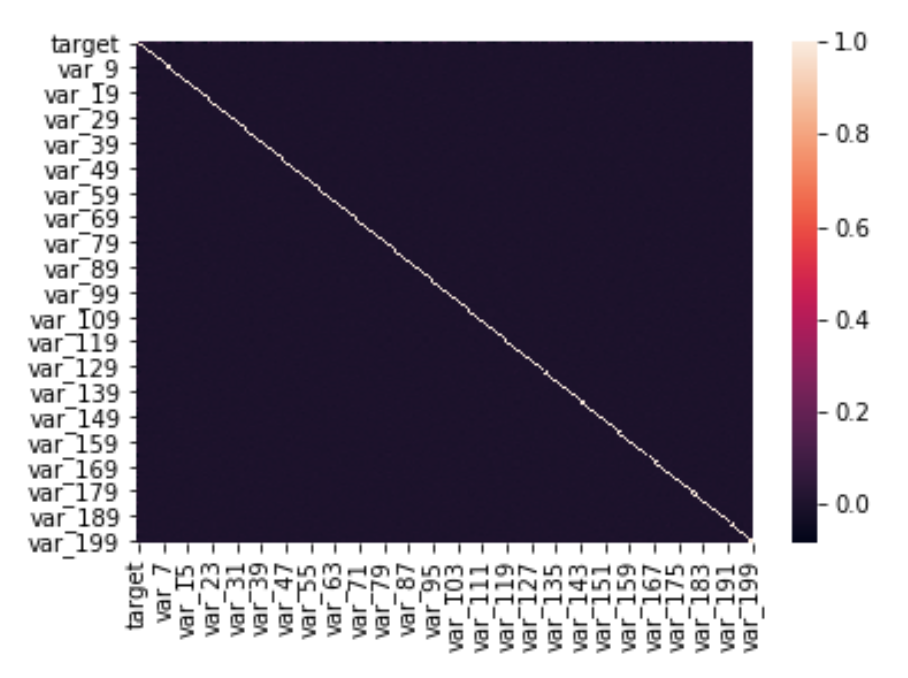
\includegraphics[width=3.6in]{project/code/heatmap.png}
  \caption{Heatmap for correlation}
  \label{fig:fig1}
\end{figure}

Since there are 200 features, plotting and examining histograms and box plots for all those features becomes a bit of difficult task. However, to make it easier, PCA was first used to identify any opportunity for reducing the dimensionality of the data. When running the PCA (figure~\ref{fig:fig2} below), it can be observed that almost all of the 200 features are required to explain 95\% of the variance. Examining the PCA plot, it is possible that the provider of the dataset already have done some preprocessing techniques, PCA possibly. 
\begin{figure}[h!]
  \centering
  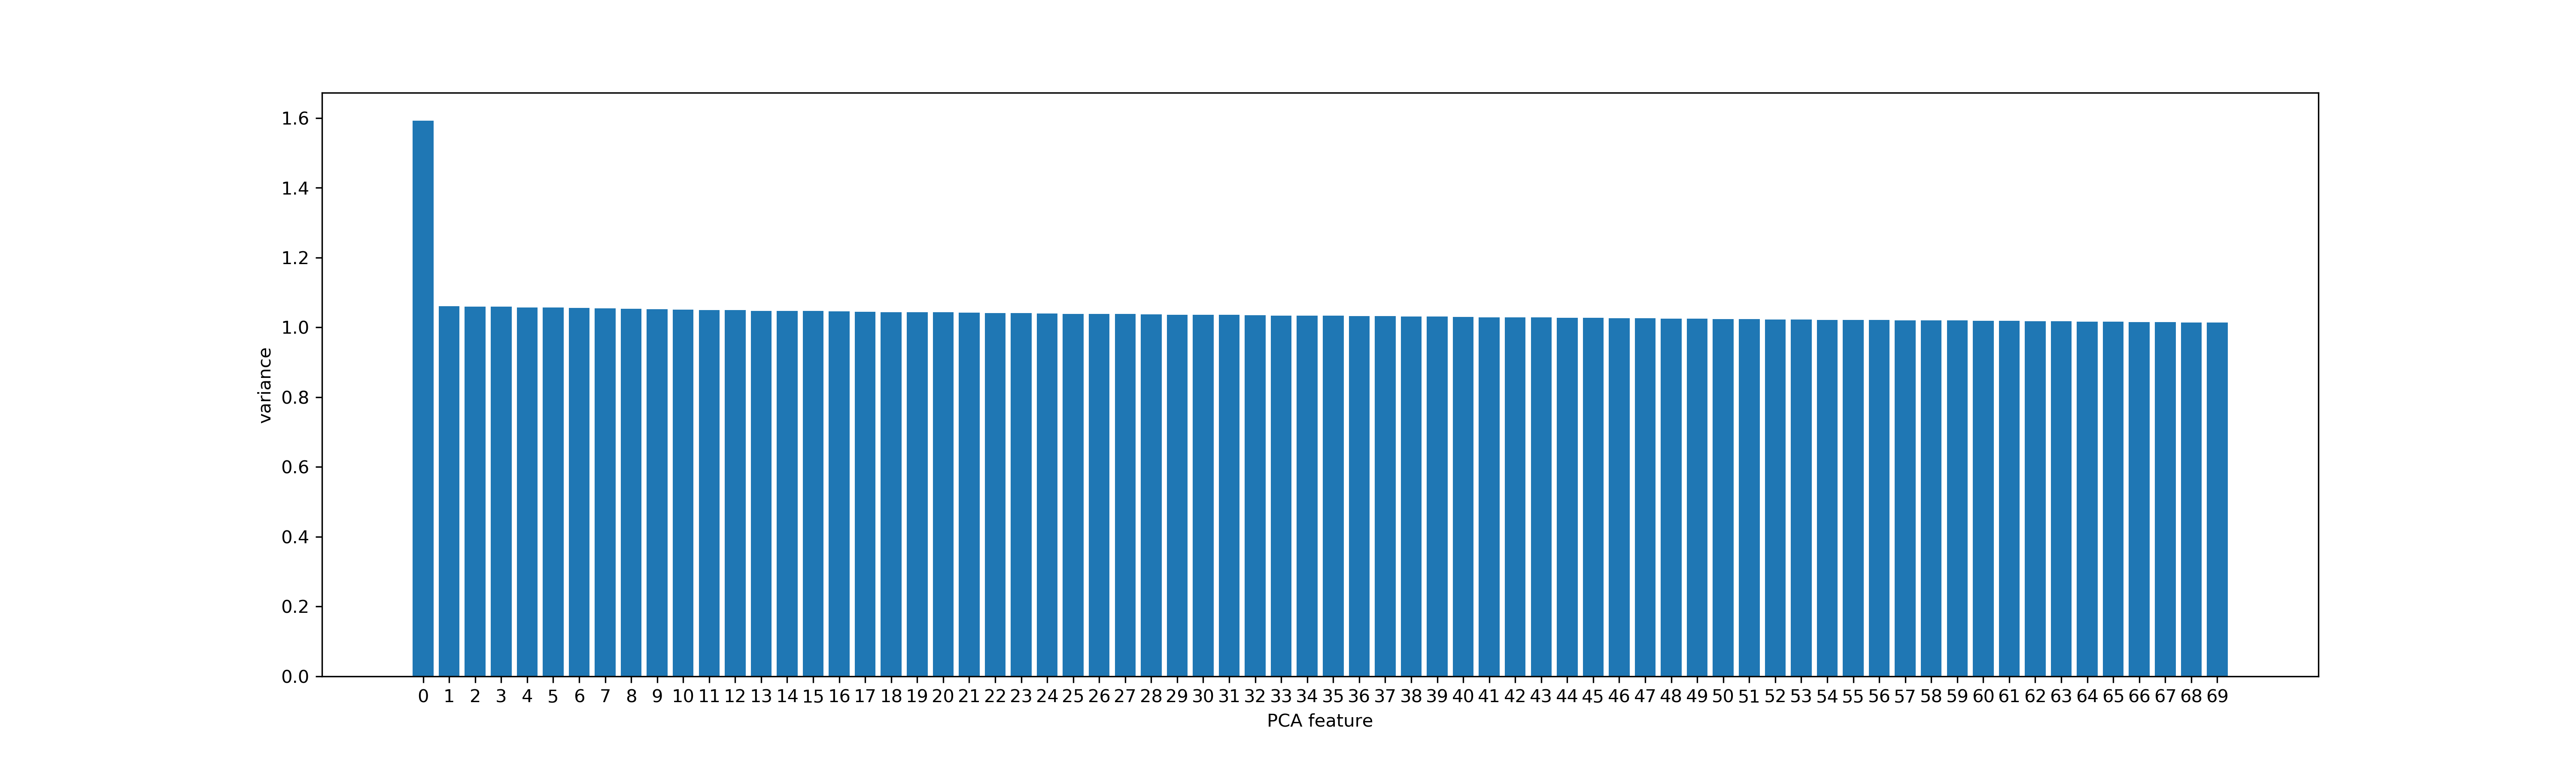
\includegraphics[width=3.6in]{project/code/1-pcafeatures.png}
  \caption{PCA}
  \label{fig:fig2}
\end{figure}
From the results above, it can be concluded that dimensionality reduction technique is not desirable in this defined problem set.

                    %%%%%%%%%%%%%%%%%%%%%%%%%%%%%%%%%%%%%%%%%%%
                    % Subsection/ Examining and Comparing Training
                    %       and Test set provided by the Competition
                    %%%%%%%%%%%%%%%%%%%%%%%%%%%%%%%%%%%%%%%%%%%

\subsection{Examining and Comparing Training and Test set provided by the Competition}

Next thing was to build a simple random forest model to extract important features and possibly providing more insights to the dataset. The reasoning behind this is to reduce the amount of time examining all the 200 features and only focus on those top 10 features. GridSearch was used to for finding the best parameters for the random forest. Figure~\ref{fig:fig3} below shows the top 10 features returned from the random forest model. 
\begin{figure}[h!]
  \centering
  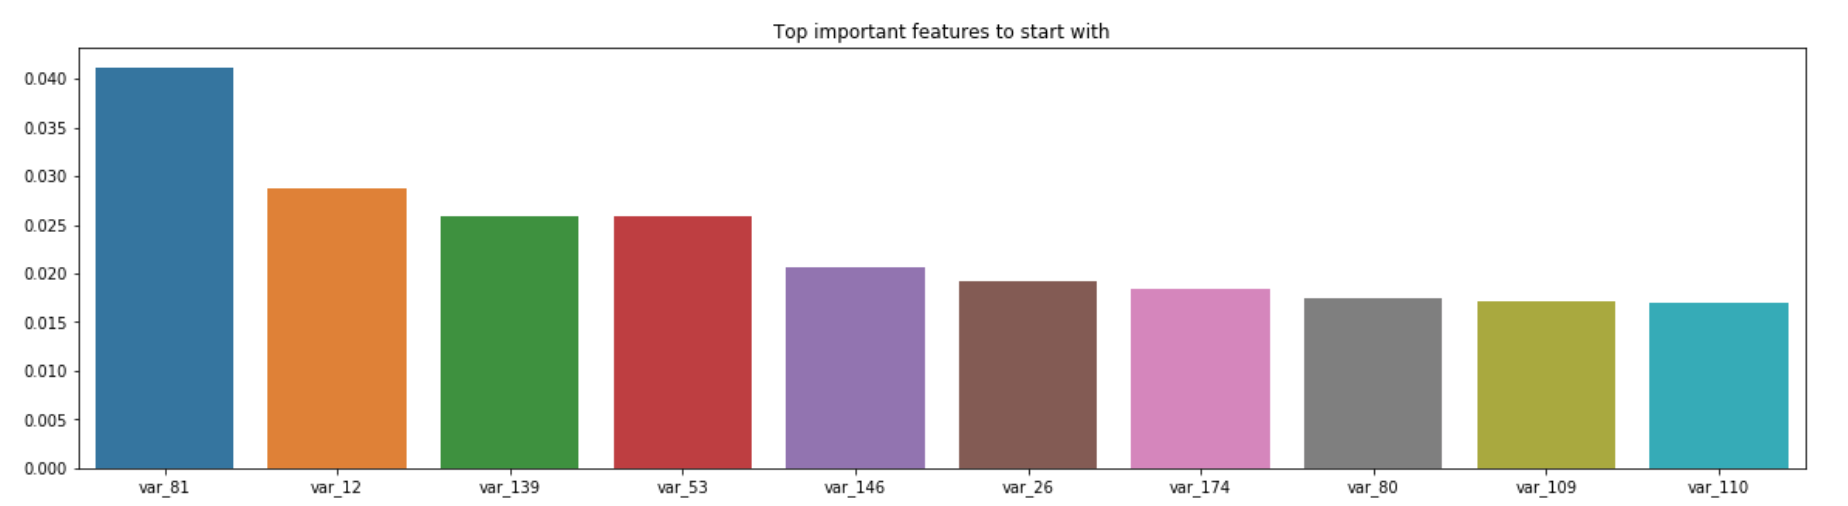
\includegraphics[width=3.6in]{project/code/important features.png}
  \caption{Important features from random forest model}
  \label{fig:fig3}
\end{figure}

Histograms were plotted for those top features as shown in figure~\ref{fig:fig4} below.

\begin{figure}[h!]
  \centering
  \includegraphics[width=3.1in]{project/code/Histograms-dist-of-features.png}
  \caption{Histograms for the top 10 features}
  \label{fig:fig4}
\end{figure}


The orange distribution is for the variable in the train dataset and the green one corresponds to the same variable in the test dataset. Comparing those features from the train and the test sets gives a conclusion can be drawn regarding the scoring for test set. More specifically, the test data does not have target so this means that prediction has to be formatted into csv file and submitted online for AUC-ROC score. However, what this distributions shows is that the train and test sets are almost similar in the distribution which means that it is possible to split the train.csv data in test and train and the cross validation (CV) score obtained in the local machine should be approximately similar to the AUC-ROC score obtained when submitted online. This give a way around the limitation of having 3 submissions a day by evaluating the model performance in the local machine using the CV score. 

                     


%%%%%%%%%%%%%%%%%%%%%%%%%%%%%%%%%%%%%%%%%%%%%%%%%%%%%%%%%%%%%%%%%%%%%%%%%%%%%%%%%%%%%%%%%%%%%%%%%%%%%%%%
% Implementation and Setup
%%%%%%%%%%%%%%%%%%%%%%%%%%%%%%%%%%%%%%%%%%%%%%%%%%%%%%%%%%%%%%%%%%%%%%%%%%%%%%%%%%%%%%%%%%%%%%%%%%%%%%%%
\section{Implementation and Setup}
The tools and experimental setup will be discussed in this section. Virtually all the models and code used to present the results in this report were developed using the Python programming language. Python has a vast ecosystem of tools and packages that allow for quick development of complex mathematical and statistical models through popular API's such as Sci-kit learn. 

Sci-kit learn was used to create the Naive Bayes and Logistic Regression model implementations. The Bayesian search used in the preliminary results was implemented using the BayesSearchCV class. This class was wrapped in a function that would take a model and search space as parameters, tune and validate the model and return the plots and metrics to benchmark the models performance. XGBoost and LightGBM have their own python packages and interfaces and were used with guidance from their documentation. 

Plotting and visualization were created using a combination of matplotlib and seaborn libraries. The Pandas module was a key component in the scientific stack for processing and managing the dataset. The dataset presented by the competition was small enough to work with completely in memory. Pandas has powerful tools to clean and permute the data to be compatible with certain models.

Final tuning for the LightGBM model was done using the library hyperopt. This optimization library allows for a Bayesian search for any problem space. The package provides an interface to save and store results from previous training. A small utility tool was developed to run the hyperopt Bayesian search and save each iteration to a save on disk. Each iteration loads the saved data and appends a new iteration upon completion.


%%%%%%%%%%%%%%%%%%%%%%%%%%%%%%%%%%%%%%%%%%%%%%%%%%%%%%%%%%%%%%%%%%%%%%%%%%%%%%%%%%%%%%%%%%%%%%%%%%%%%%%%
% Results and Discussion
%%%%%%%%%%%%%%%%%%%%%%%%%%%%%%%%%%%%%%%%%%%%%%%%%%%%%%%%%%%%%%%%%%%%%%%%%%%%%%%%%%%%%%%%%%%%%%%%%%%%%%%%
\section{Results and Discussion}
The results of the methods outlined in methodology are described in this section. Overall, the four initial models performed decently well. 

\subsection{Baseline Models}

Four baseline models were evaluated to determine which methods perform well on the dataset. The four classifiers trained were Naive Bayes, Logistic Regression, XGBoost and LightGBM as outlined in the methodology section. In order to benchmark each model all the classifiers were trained on a subset of the provided "train.csv". The data was first down-sampled to allow for each representation of both labels. The inputs to the classifiers were also normalized using z-score. The hyper-parameters for each model were tuned using Bayesian cross validation. 

The Naive Bayes algorithm was tuned over 100 iterations using Bayesian search and had only one hyper-parameter, "var-smoothing". The utility script developed ran the iterations and evaluated the performance of the best performing parameters in the search. Figure~\ref{fig:prelim-NB} shows the result of the preliminary model showing the Receiver Operating Characteristics Area Under The Curve (AUC\_ROC), precision-recall (PR) curve, and the resulting confusion matrix with classification report. 

The classifier performed well with a macro average f1-score of 0.81. The AUC\_ROC curve had an area of 0.88 and indicates that the classifier has a decent amount of separation between the class labels. The PR curve is generally more representative of performance when evaluating against a dataset with imbalanced class labels. The recall values presented in the classification report indicate that the model generalized well and did not bias predictions to one class over the other.

\begin{figure}[h!]
  \centering
  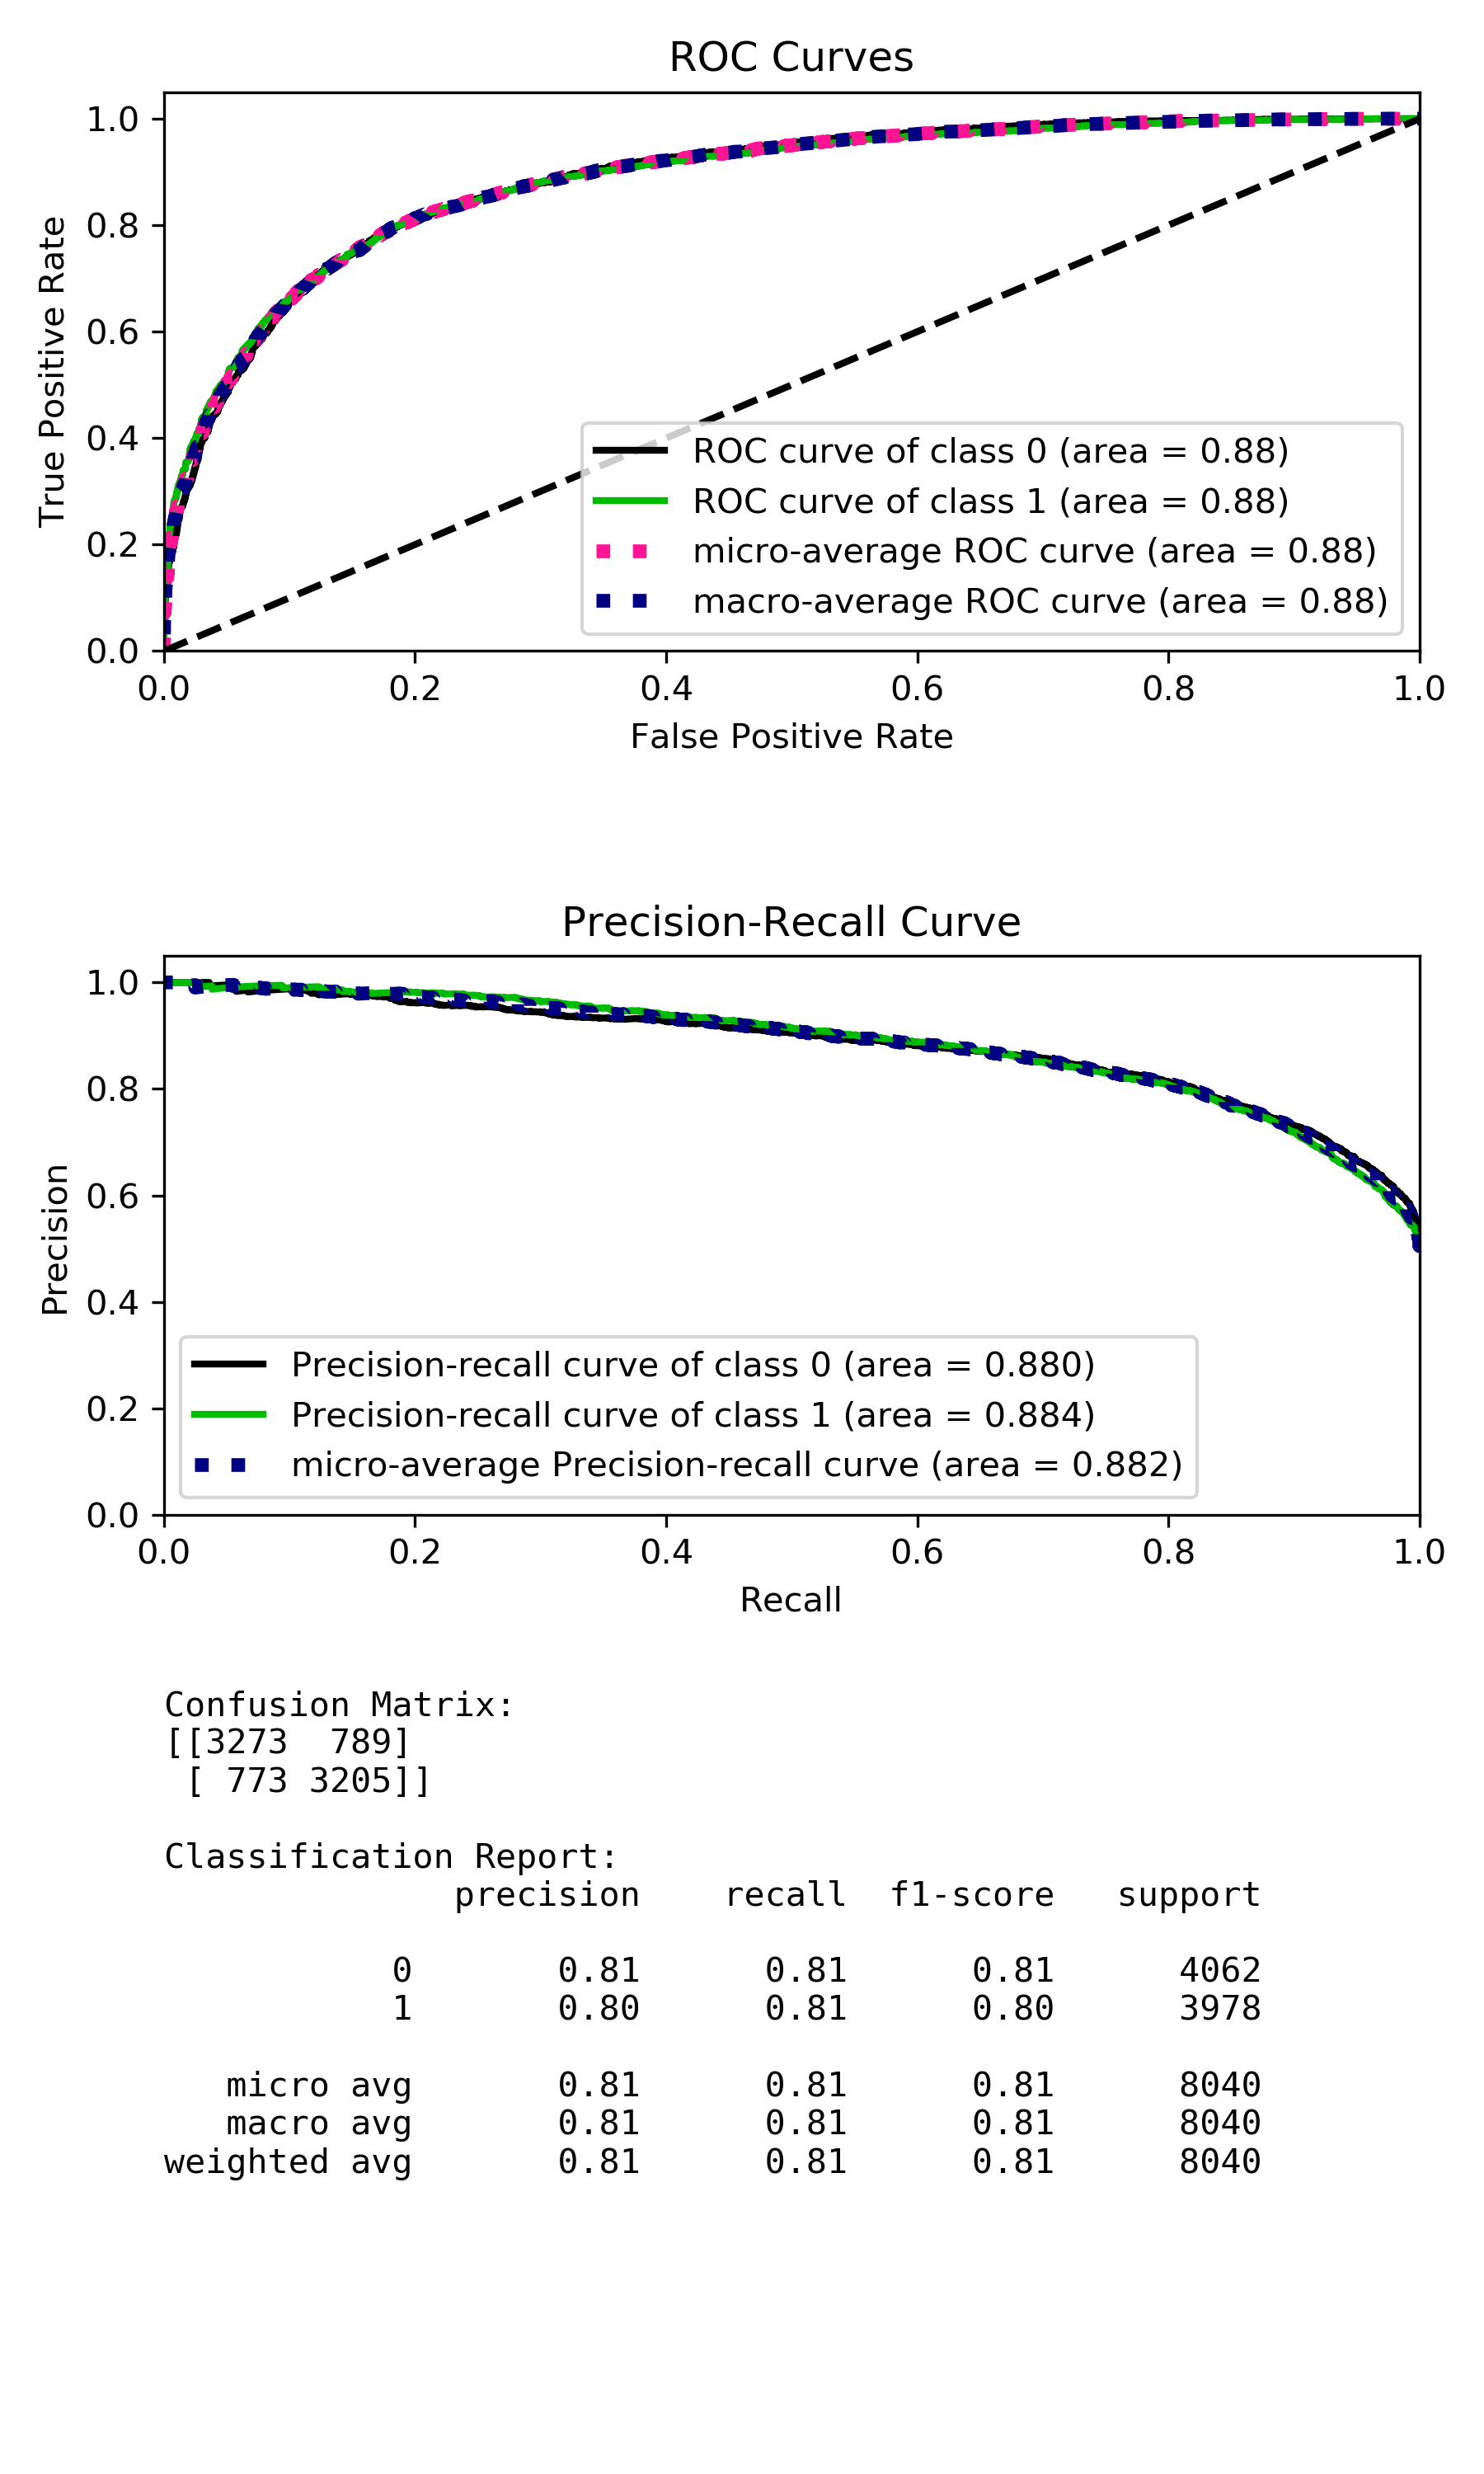
\includegraphics[width=3.6in]{project/code/preliminary-naivebayes-downsampled.png}
  \caption{Baseline model performance for Naive Bayes classifier}
  \label{fig:prelim-NB}
\end{figure}

The second model evaluated was a Logistic Regression classifier. Again the model was tuned using the Bayesian cross-validation technique. Two hyper-parameters were searched for: "C" or the inverse regularization term and solver. After 100 iterations, the optimal values found were C at $1.05e^{-4}$ \expnumber{1.05}{-4} using the "saga" solver. Figure~\ref{fig:prelim-logreg} displays the same performance metrics as before. The logistic regression model performed slightly worse than the Naive Bayes classifier with a macro f1-score of 0.77 and AUC\_ROC of 0.85. 

The last two models were both random forest implementations using gradient boosting, one using the XGBoost implementation and the other using LightGBM. Due to the increases computational demand the cross validation for each of these methods was only done over 20 iterations. It is difficult to know if the paramters searched were optimal, however, the performance of the two models were similar to the benchmarks provided by Naive Bayes and Logistic Regression.

The LightGBM model performed almost equivalently to XGBoost as seen in the performance results shown in Figure~\ref{fig:prelim-lgbm} and Figure~\ref{fig:prelim-xgboost} respectively. XGBoost had an AUC\_ROC score of 0.89 and f1-macro average of 0.77 while LightBGM had an AUC\_ROC of 0.88 with f1-macro of 0.80.

These results served as a starting point to conduct additional investigations to try and improve performance of the model on the submission dataset. While the models results were similar, a lot factors contribute to a model's performance. It is possible that the under sampled data used to train the random forest classifiers did not have enough samples to allow the model to generalize to the submission dataset optimally. It was also possible that the parameters tuned need to be manually adjusted or searched over a larger parameter space.

\subsection{Improving Baseline Models}
\subsubsection{Up-sampling using SMOTE}
To test the theory that increased data samples could allow certain models to generalize more effectively we trained the baseline models once again using the parameters found initially. We kept all constants the same except the inputs to the models. The results of the trial can be seen in Table~\ref{table:tab2}. None of the classifiers performed better using the up-sampled data and XGBoost and Naive Bayes in particular resulted in no ability to distinguish class label. There are could be a few reasons for this result, first, the up-sampling techniques could have made new data points with too much similarity to the original samples. This would cause the models to over-fit the training data and lose separation between the class labels. Second, the models were trained using the hyper-parameters found in the baseline model benchmark using the down-sampled data, it is possible that these hyper-parameters are not optimal for the training input. Lastly, the method by which the samples were duplicated could have been inappropriate for the data. K-nearest neighbours was used to create the new samples, modifications to the value of K were not explored but could have altered the results obtained.

\begin{table}
\begin{tabular}{|{2.0cm}||p{2.0cm}|p{2.0cm}}
\hline
\multicolumn{3}{|c|}{Baseline Models Up-sampling vs Down-sampling} \\
\hline
Classifier & SMOTE Up-sampled AUC\_ROC & Down-Sampled AUC\_ROC\\
\hline
Naive Bayes         & 0.50 & 0.88 \\
Logistic Regression & 0.68 & 0.85 \\
XGBoost             & 0.50 & 0.89 \\
LightGBM            & 0.70 & 0.88 \\
\hline
\end{tabular}
\caption{Baseline model performance on Up-sampled vs Down-sampled data}
\label{table:tab2}
\end{table}

\subsubsection{Ensembling Baseline Models}
Another attempt to improve the accuracy from the initial benchmark obtained with the baseline models was to ensemble the four classifiers together. Two simple methods were attempted: averaging and voting. Overall, no improvement or degradation was seen using the ensembled classifiers. This inconclusive results do not mean the technique is not applicable, however, adjustments would have to be made to better use this strategy. 

The four classifiers may be predicting samples similarly and have a similar probability distribution of the predictions. In this case, new insights would not be available from ensembling because each of the individual distributions overlap. This could change as better hyper-parameters are found or if new features are designed and model accuracies improve. Individual models would ideally be better at predicting certain samples than others and an improved ensembling architecture could take advantage this characteristic.

\subsection{Extensive Hyper-Parameter Tuning for the LightGBM Model}
Here we present the results of an extensive hyper-parameter search over the LightGBM's parameter space. Since the previous attempts did not yield favourable results, focus was placed primarily on a single model implementation of LightGBM. LightGBM has the advantage of training models quicker than XGBoost however, it requires more data to be successful. LightGBM has a built in parameter flag named "is\_balanced" that can be used compensate for unbalanced datasets.

An in depth Bayesian hyper-parameter search was performed using the full dataset. The search iterated over 700 possible hyper parameter configurations over multiple days. Twelve key parameters were searched chosen according to recommendations found in the LightGBM documentation~\cite{lightgbm_documentation}. These parameters are:
\begin{itemize}
\item min\_sum\_hessian\_in\_leaf
\item bagging\_fraction
\item bagging\_freq
\item min\_gain\_to\_split
\item boosting\_type
\item num\_leaves
\item learning\_rate
\item subsample\_for\_bin
\item min\_child\_samples
\item lambda\_l1
\item lambda\_l2
\item feature\_fraction
\end{itemize}

Number of leaves is an important parameter to tune when using LightGBM. Number of leaves controls the complexity of the model. The value must be large enough to learn the features of the data, but too many leaves could result in over fitting. Figure~\ref{fig:lgbmtuning_numleaves} shows a plot of the distribution of values tested for number of leaves during the hyper parameter search

\begin{figure}[h!]
  \centering
  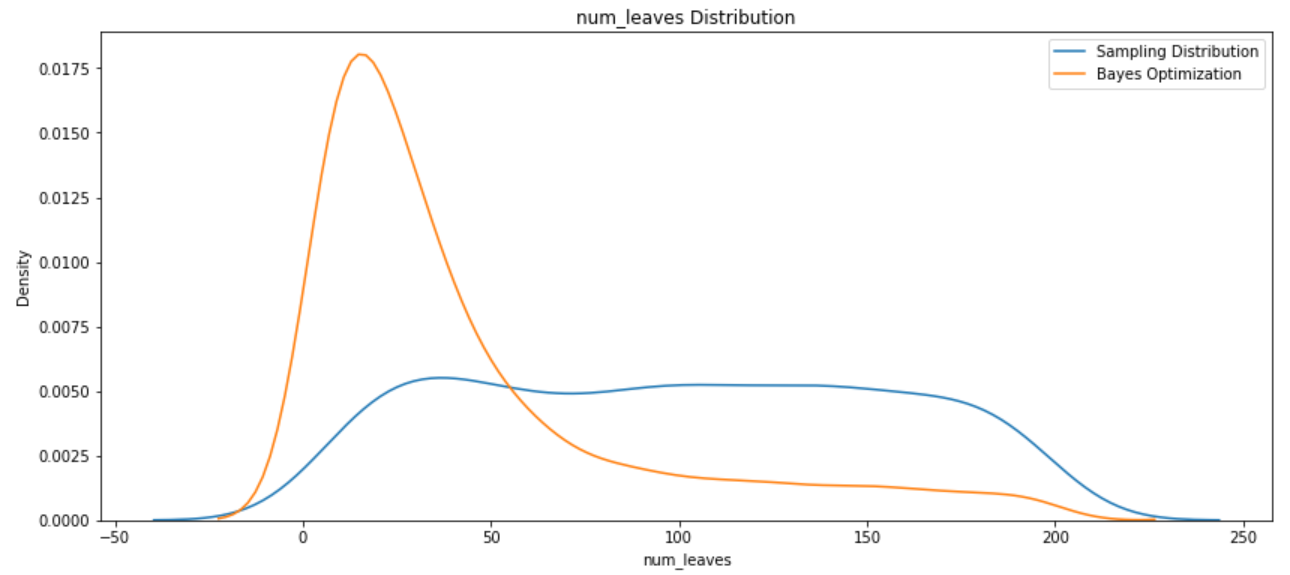
\includegraphics[width=3.6in]{project/code/results/num-leaves-distplot.png}
  \caption{Distribution of search values for "num\_leaves" parameter}
  \label{fig:lgbmtuning_numleaves}
\end{figure}

We can see that the Bayesian search is selecting values that differ from the sample distribution but have a higher likelihood of improving performance. After the search was completed and the optimal parameters were tuned the model performed better than all baseline models. The tuned LGBM model resulted in an AUC\_ROC score of 0.896. The train time for the model with optimal parameters was 300 seconds and contained 5001 estimators. This model was then used to evaluate the submission dataset and returned a result of 0.898 on the Kaggle leaderboard.



%%%%%%%%%%%%%%%%%%%%%%%%%%%%%%%%%%%%%%%%%%%%%%%%%%%%%%%%%%%%%%%%%%%%%%%%%%%%%%%%%%%%%%%%%%%%%%%%%%%%%%%%
% CONCLUSION
%%%%%%%%%%%%%%%%%%%%%%%%%%%%%%%%%%%%%%%%%%%%%%%%%%%%%%%%%%%%%%%%%%%%%%%%%%%%%%%%%%%%%%%%%%%%%%%%%%%%%%%%

\section{Conclusion}
In this project, we analyzed the Santander's bank data set to identify which customer will make a transaction irrespective of money transacted,we setup preliminary models by  classifying the data using different machine-learning algorithms(Naive Bayes ,Logistic Regression, XGBoost, and LGBM) to predict which customer makes a transaction, then we evaluated each model performance regarding its accuracy, precision, Recall, F-measure to find the best classifier. This results formed our benchmark on which we built upon to push performance further by developing hypothesis with a well tested analysis on which performance was eventually evaluated.We found that the LightGBM with extensive hyper-parameter tuning offered the highest performance(89.6\%) with efficient train time(300sec) which made it the best model to analyze the dataset.

Data science and machine learning is an iterative process and many modifications could be made to the models and techniques presented in this paper. Our future work would involve exploring the efficacy of new models, such as, neural networks and attempting to extract useful features use more elaborate feature engineering techniques.



% IEEE Xplore\textregistered\ at no charge, \underline{http://graphicsqc.ieee.org/}, allows authors to 


\appendices



\clearpage{}
\section{Preliminary Model Results}
\begin{figure}[h!]
  \centering
  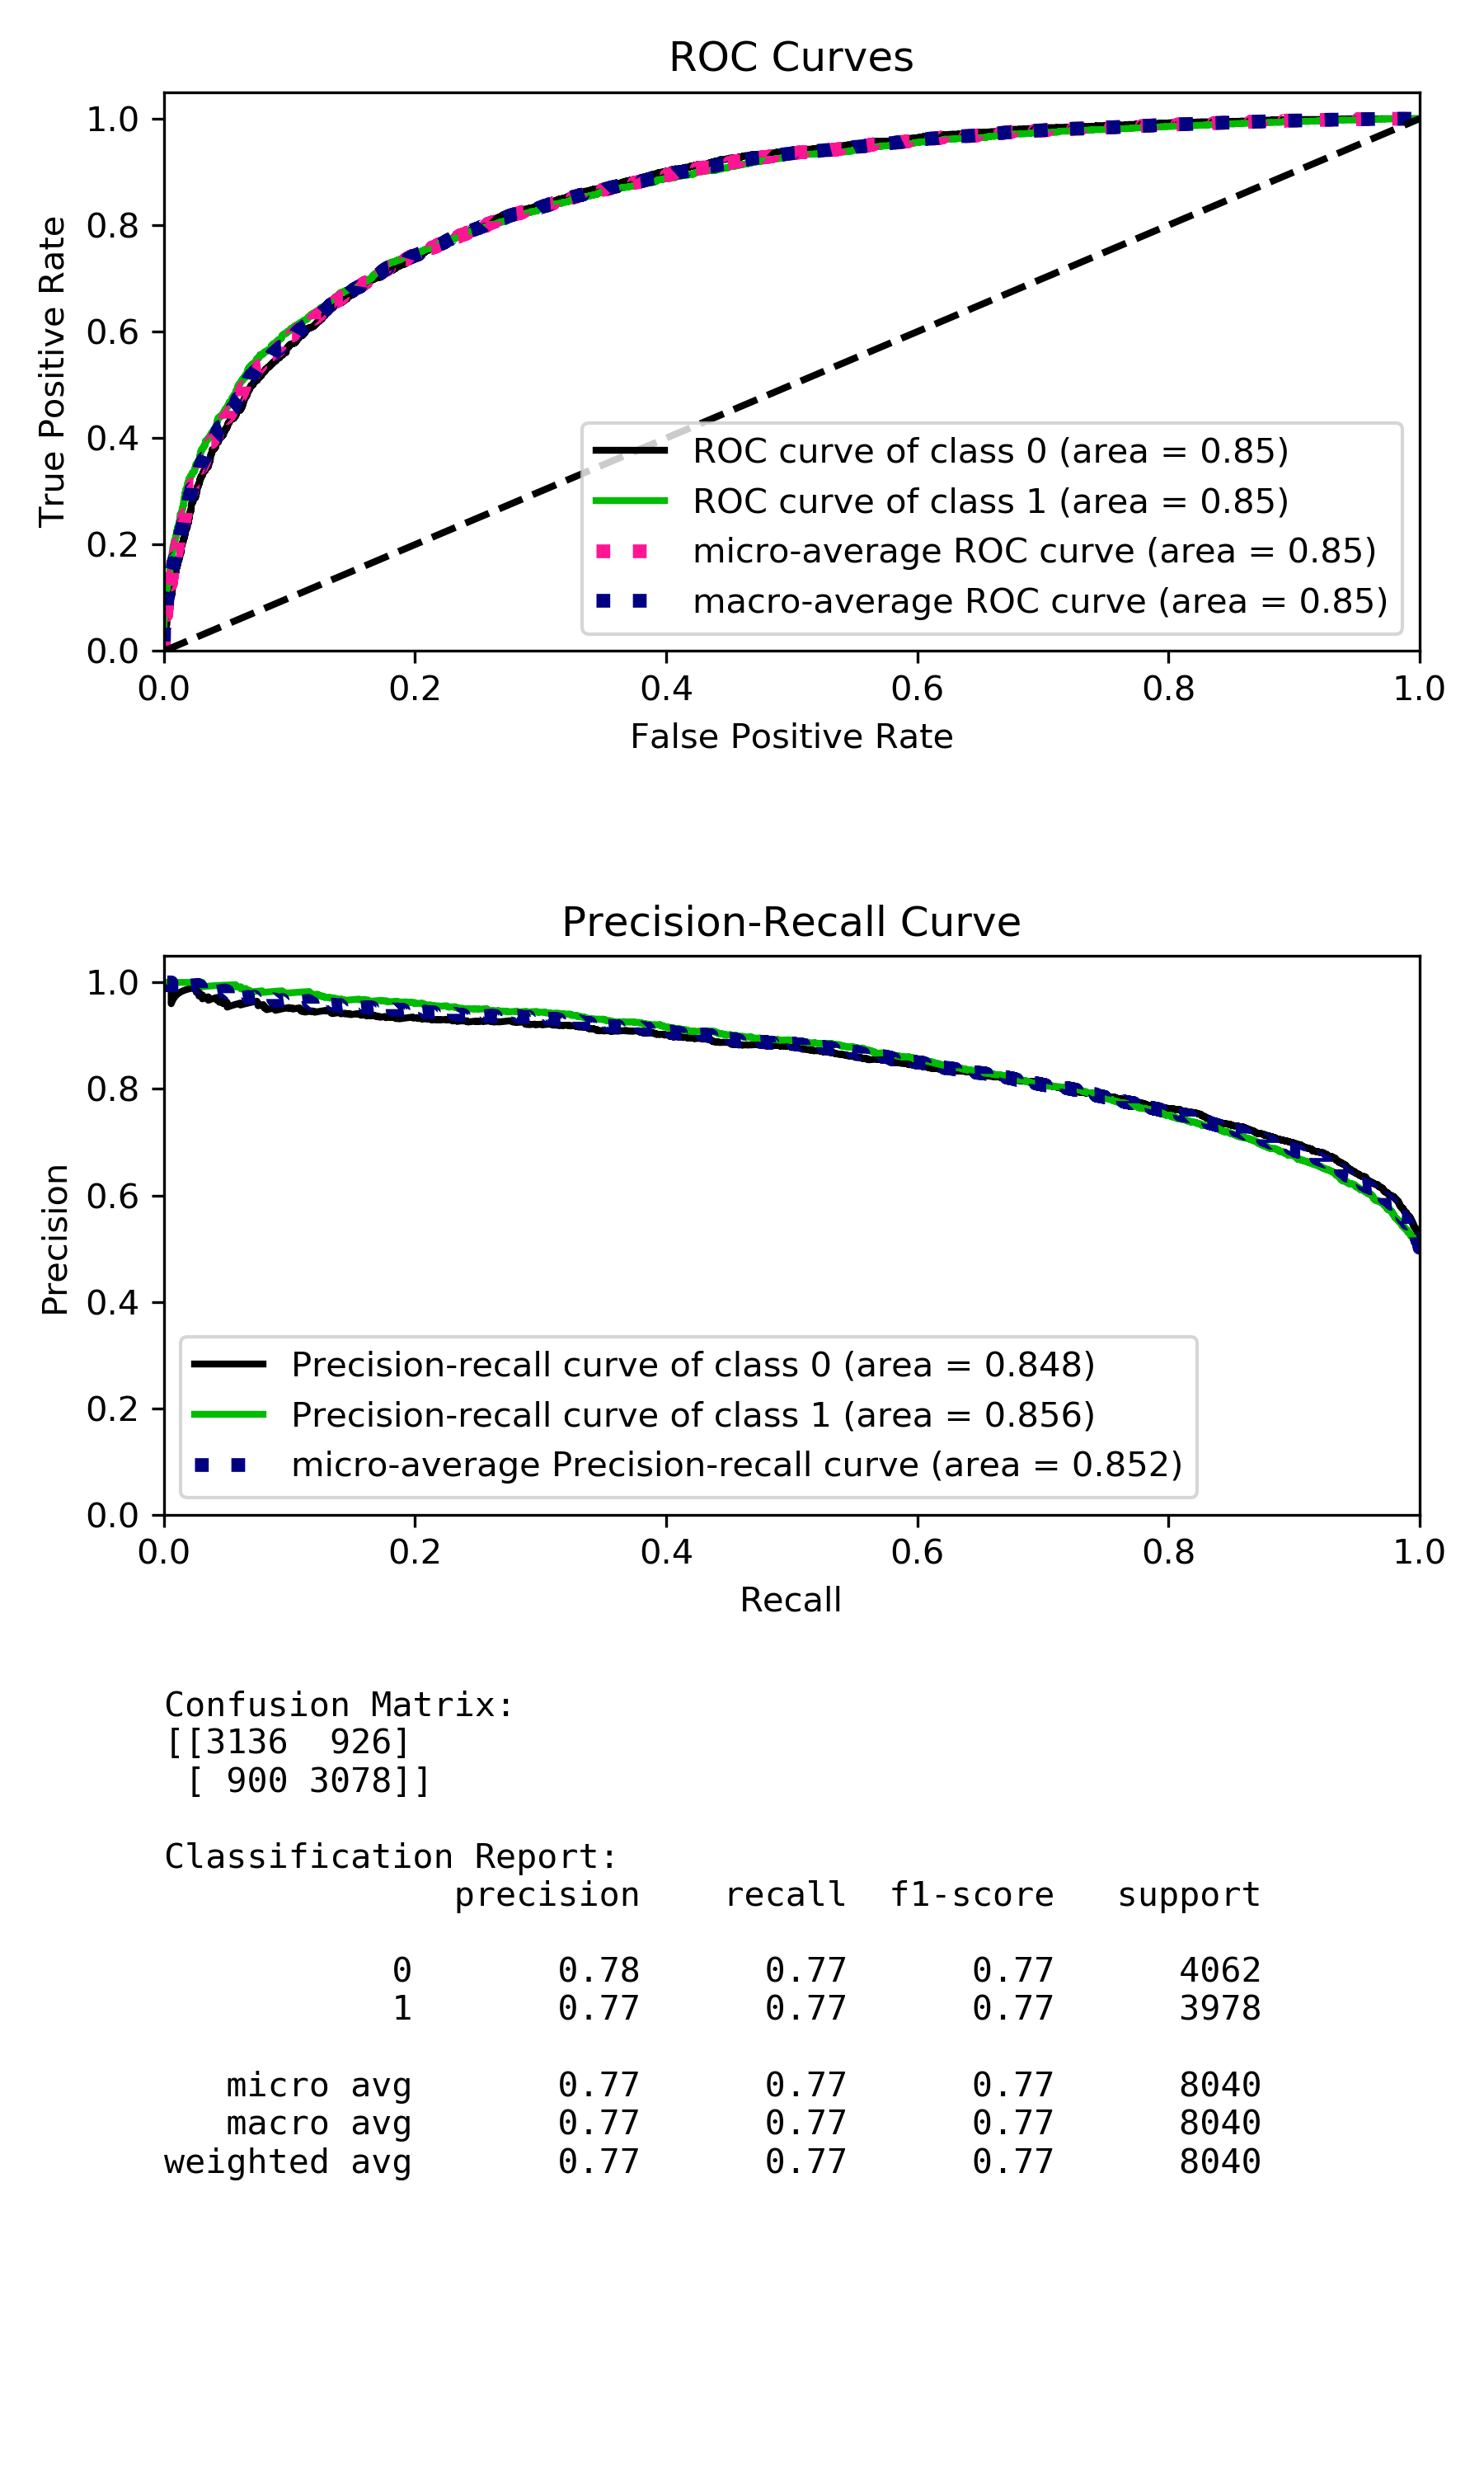
\includegraphics[width=3.1in]{project/code/preliminary-logregression-downsampled_f1score.png}
  \caption{Baseline model performance for Logistic Regression classifier}
  \label{fig:prelim-logreg}
\end{figure}

\begin{figure}[h!]
  \centering
  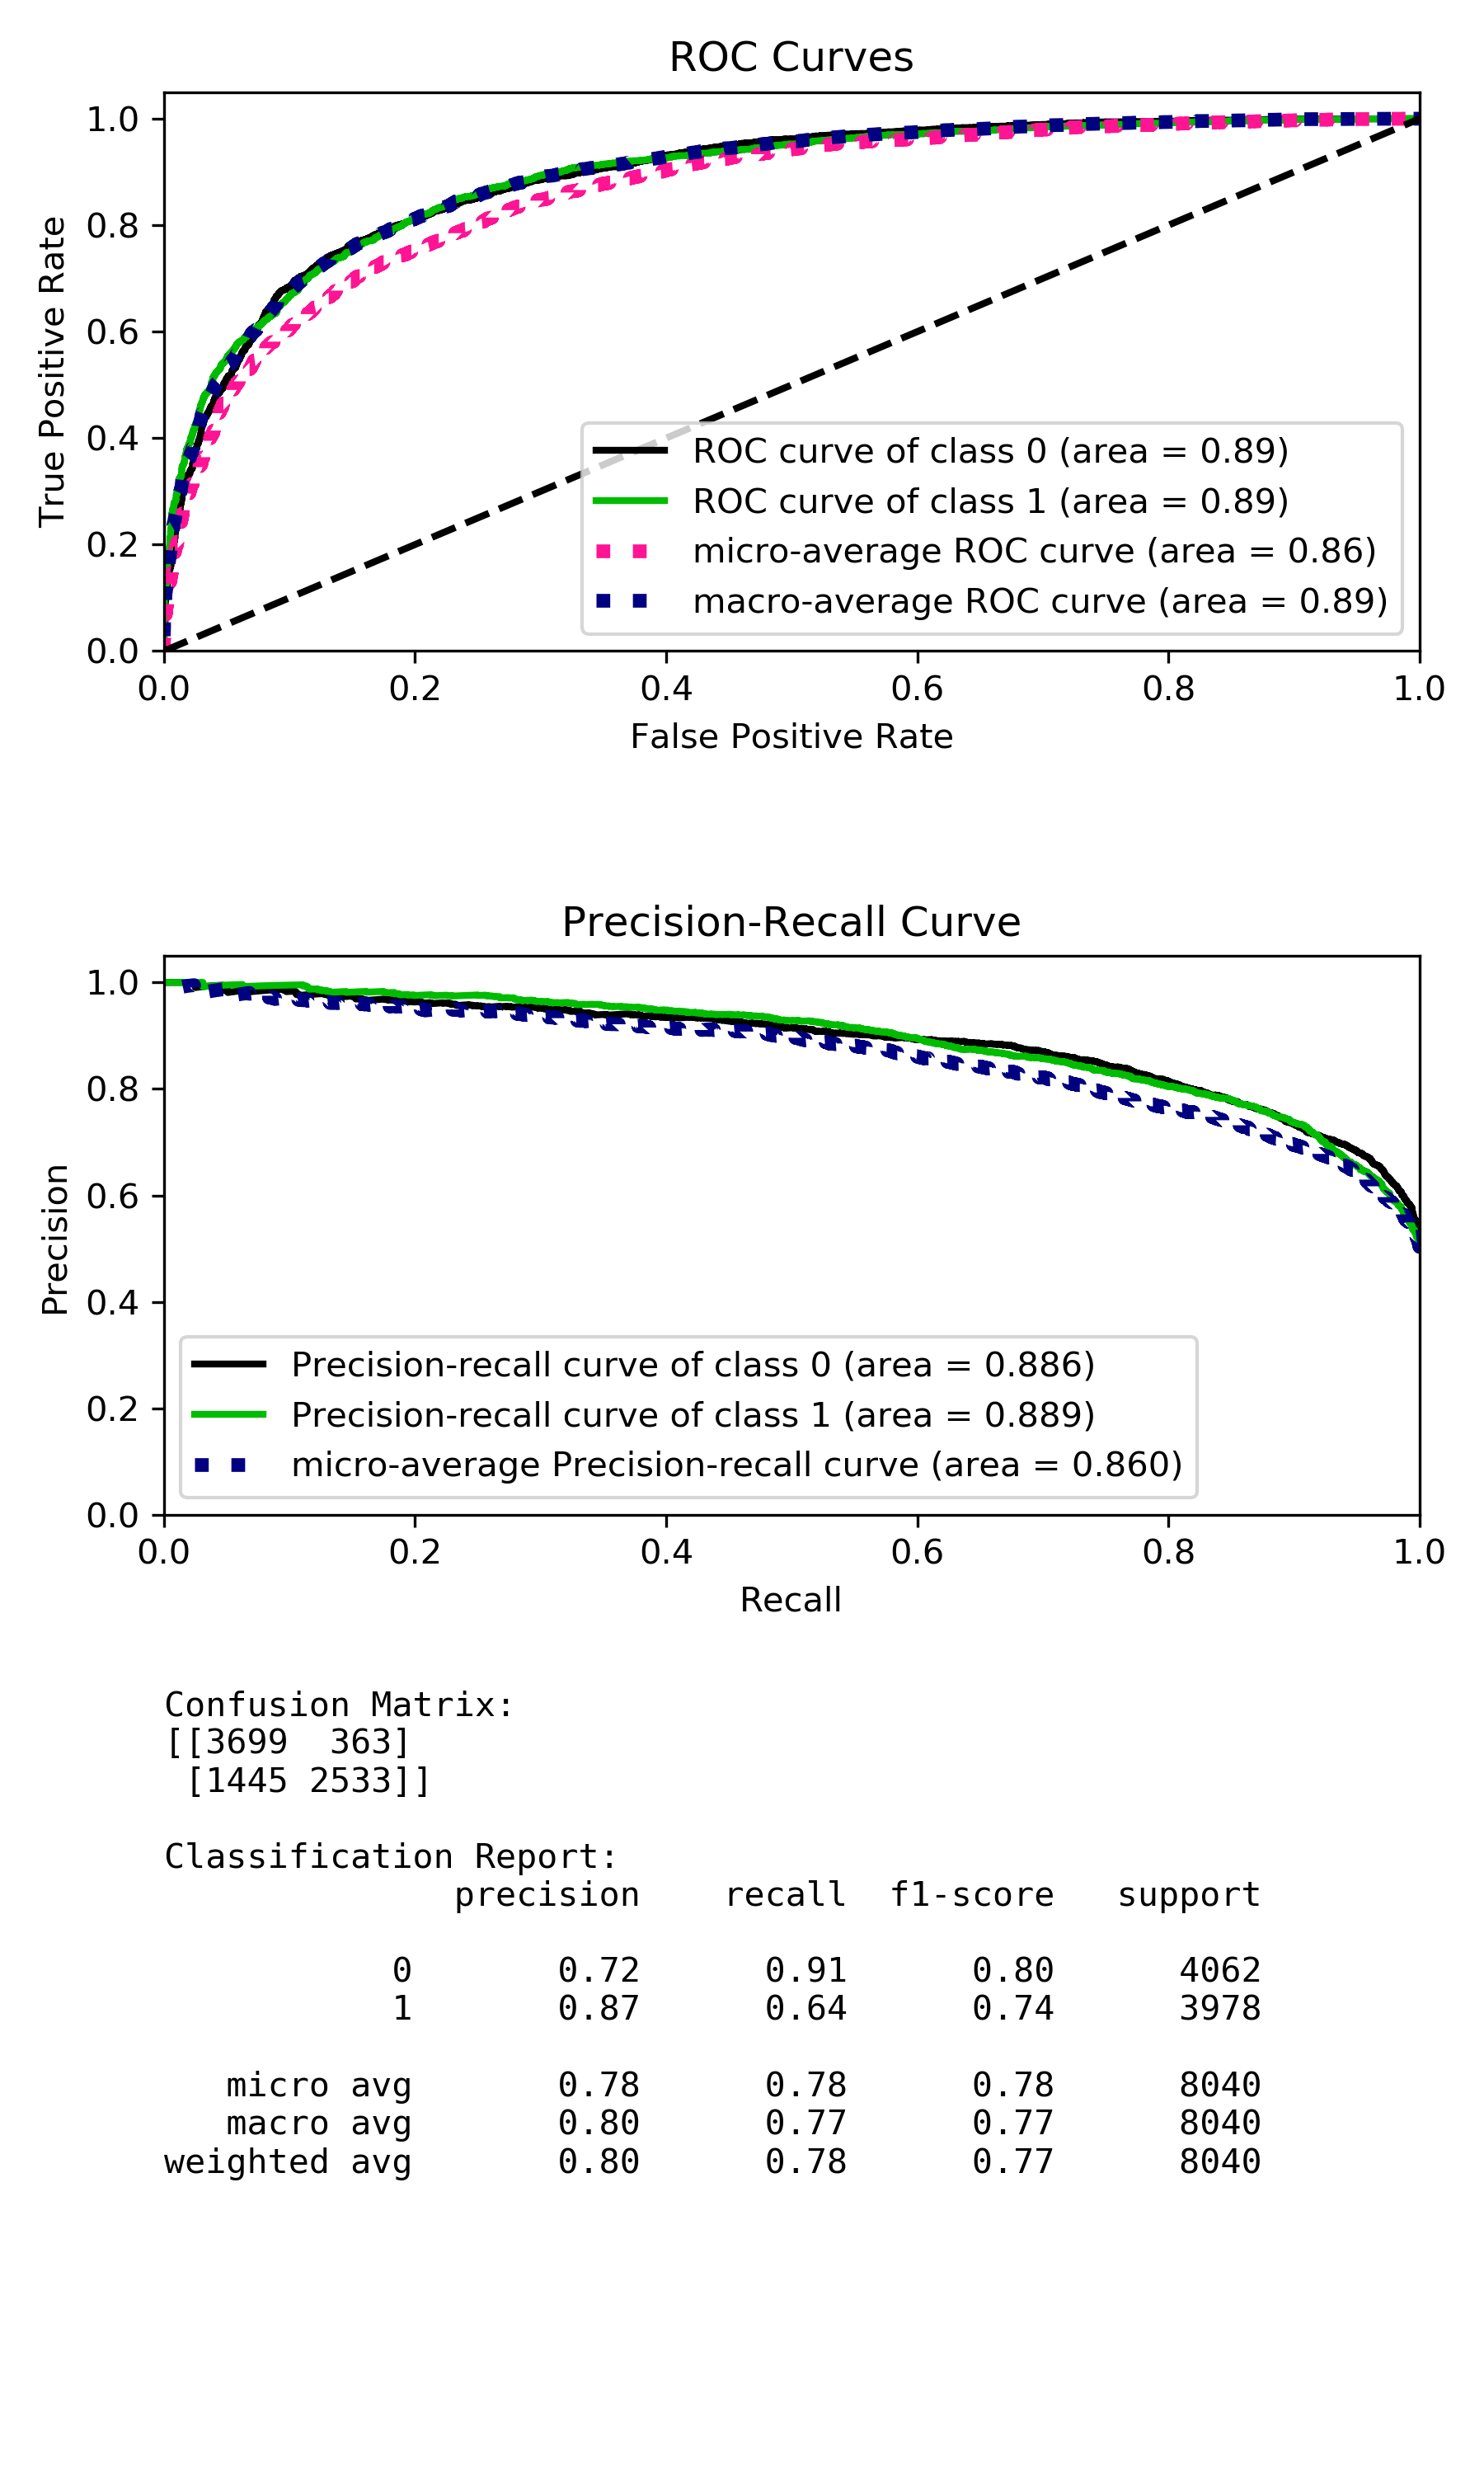
\includegraphics[width=3.1in]{project/code/preliminary-xgboost-downsampled.png}
  \caption{Baseline model performance for XGBoost classifier}
  \label{fig:prelim-xgboost}
\end{figure}

\begin{figure}[h!]
  \centering
  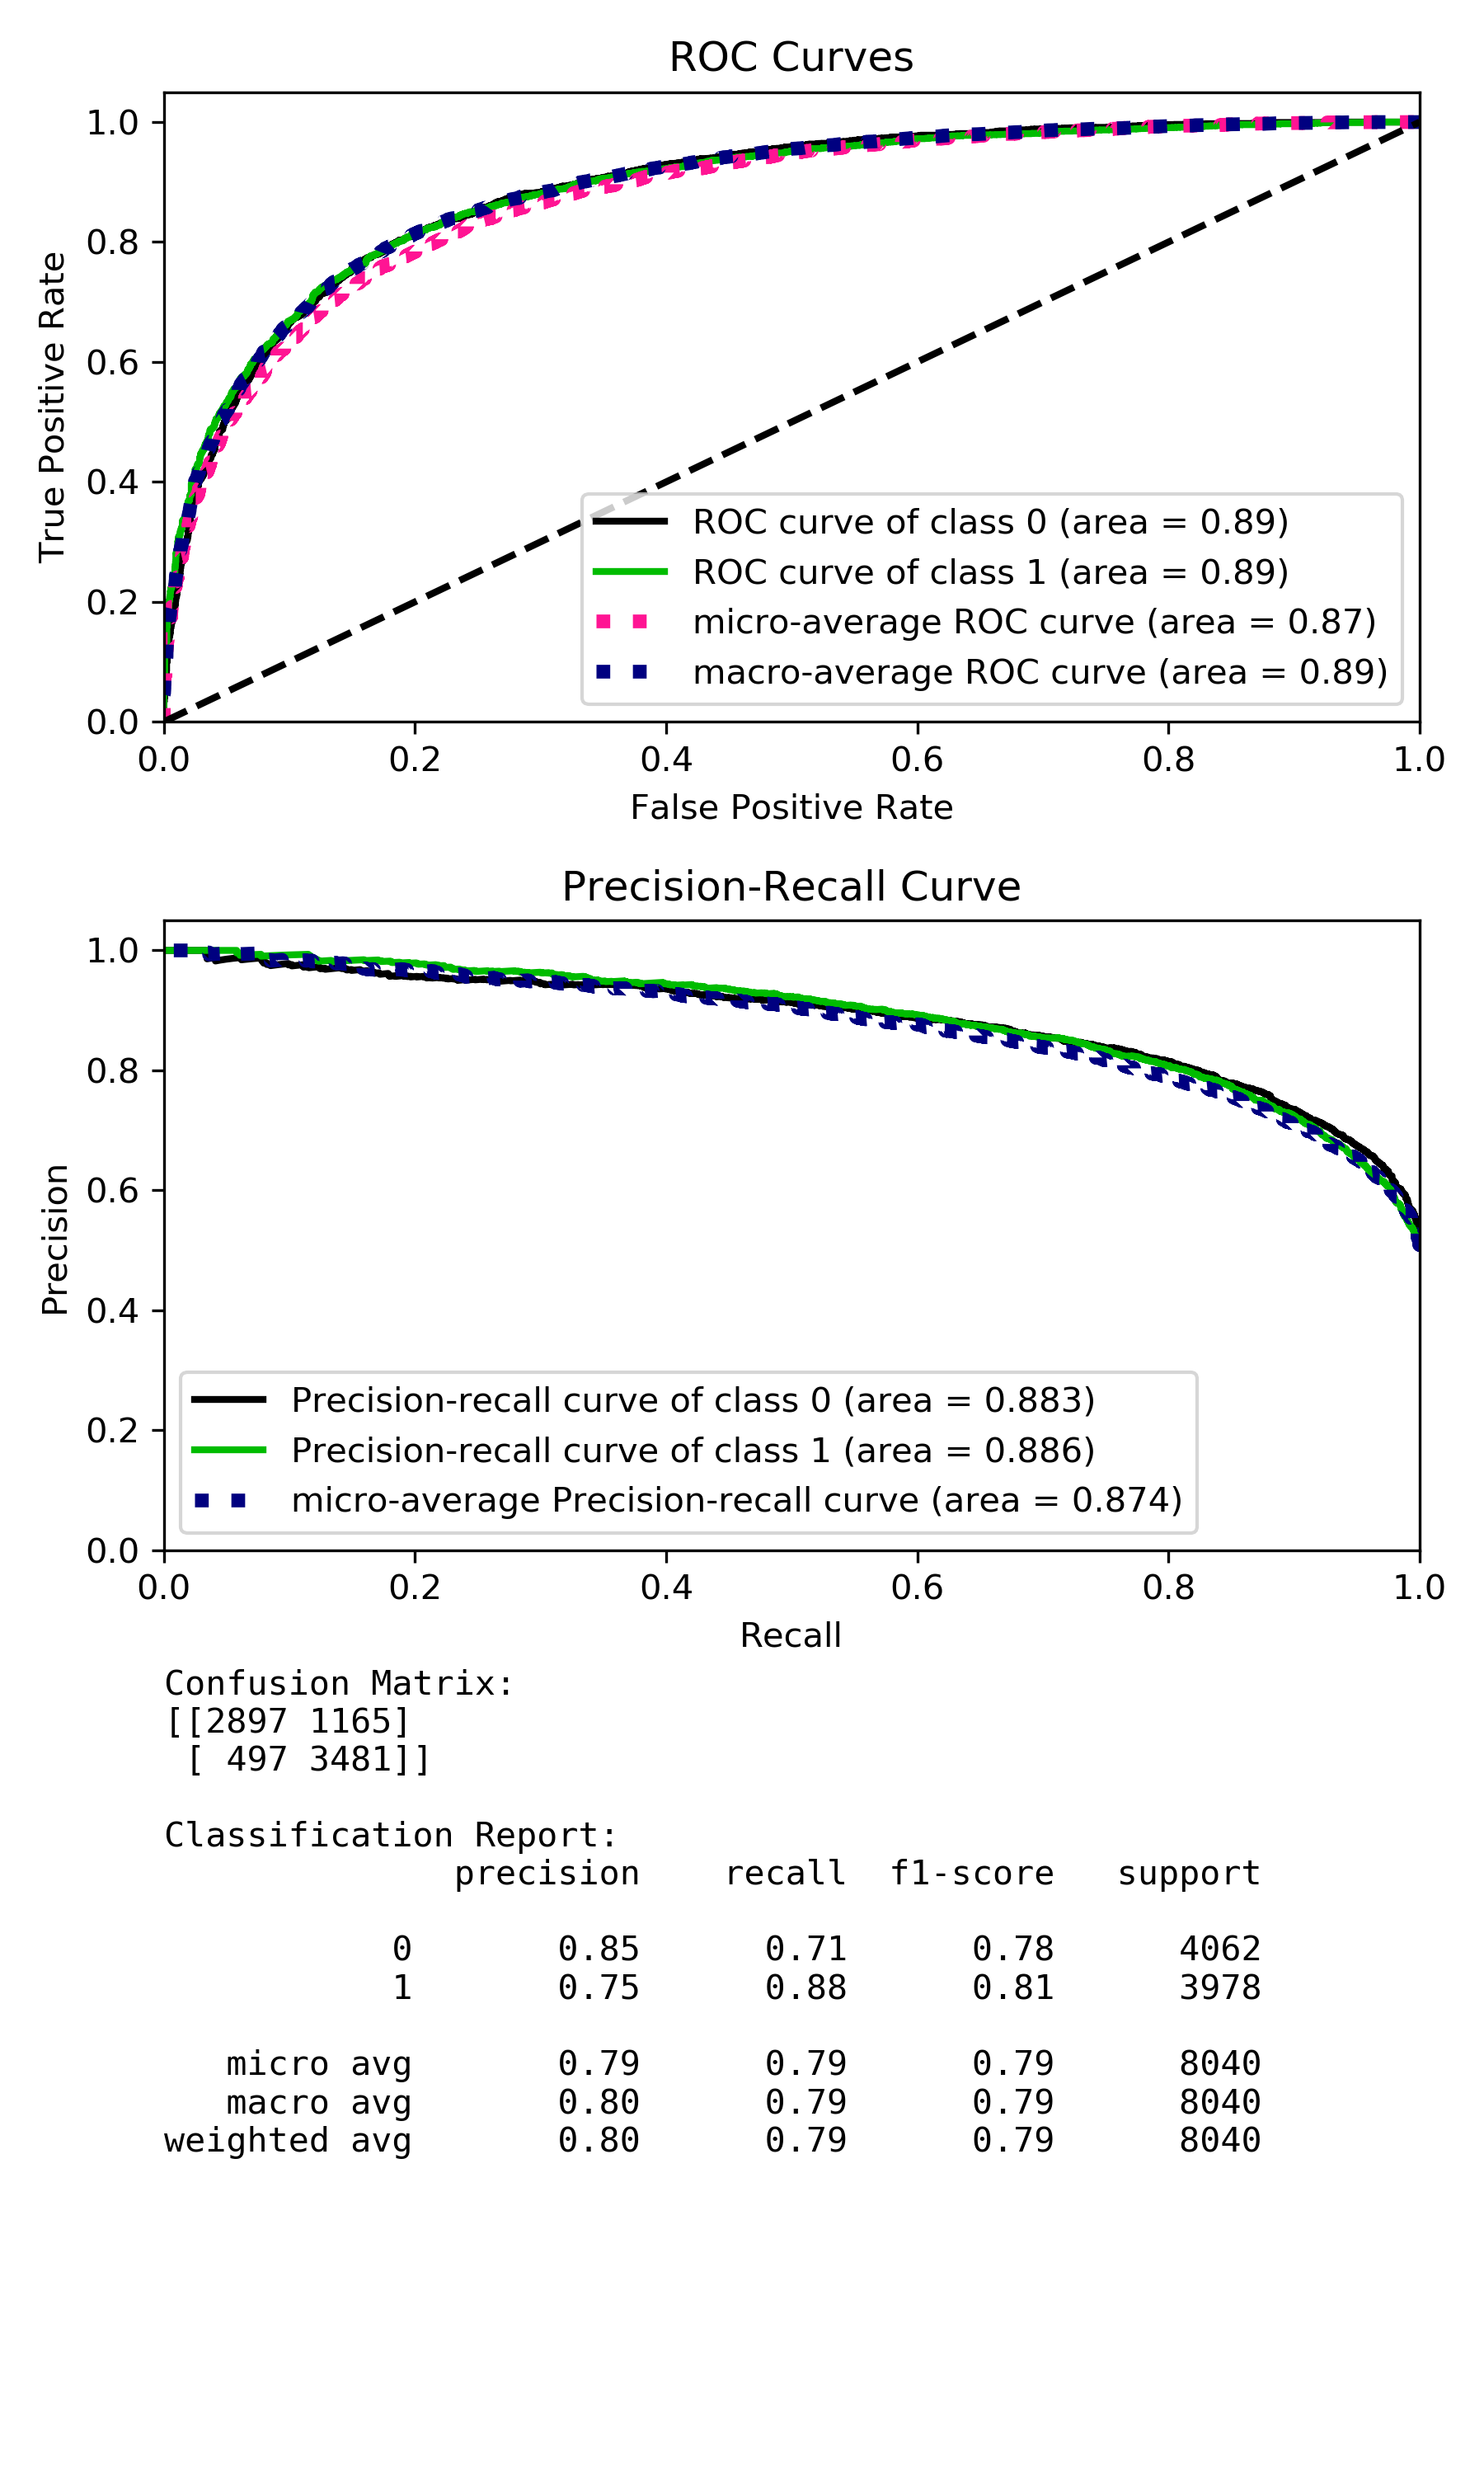
\includegraphics[width=3.1in]{project/code/preliminary-lightGBM-downsampled.png}
  \caption{Baseline model performance for LightGBM classifier}
  \label{fig:prelim-lgbm}
\end{figure}




\section*{References and Footnotes}
\subsection{References}

\nocite{*}
\bibliographystyle{IEEEtran}
\bibliography{ref}



\end{document}
